\documentclass[10pt,a4paper]{article}
\usepackage[T1]{fontenc}
\usepackage[utf8]{inputenc}
\usepackage[english]{babel}
\usepackage{lmodern}
\usepackage[margin=22mm]{geometry}
\usepackage{xcolor,array,tabularx,booktabs,amsmath,enumitem,tikz}
\usetikzlibrary{arrows.meta,positioning}
\definecolor{ink}{HTML}{303030}
\definecolor{pale}{HTML}{F2F2F2}
\definecolor{accent}{HTML}{E3EAF0}
\setlength{\parindent}{0pt}
\setlength{\parskip}{6pt}
\setlength{\emergencystretch}{2em}
\renewcommand{\arraystretch}{1.2}
\setlist[enumerate]{leftmargin=*,itemsep=3pt,topsep=3pt}
\newcolumntype{Y}{>{\raggedright\arraybackslash}X}
\newcolumntype{P}[1]{>{\raggedright\arraybackslash}p{#1}}
\newcommand{\code}[1]{\texttt{#1}}
\newcommand{\topic}[1]{\vspace{5pt}{\large\bfseries #1}\par}
\pagestyle{plain}
\tikzset{box/.style={draw=ink,rounded corners=2pt,fill=pale,align=center,font=\small,inner sep=6pt},arr/.style={-{Latex[length=2mm]},thick,draw=ink}}
\begin{document}
\vspace*{40mm}
\begin{center}
{\Large Management of Telecom Projects}\par\vspace{8pt}
{\large Task 11: Unicode File Transfer}\par\vspace{18pt}
Guillem Moreno\\[4pt]
Team C\\[12pt]
October 2026
\end{center}
\vfill
\clearpage

\topic{1. Input format and transfer method}
The competition supplies Unicode text files, but does not specify their encoding, byte order or use of a byte order mark. The transfer method must therefore preserve files encoded in UTF-8, UTF-16 or UTF-32 without requiring their interpretation.

The file is read in binary mode into a \code{uint8\_t} buffer. Each read returns $n$ bytes, which are passed unchanged to the transport. A byte is an 8-bit value from 0 to 255. Buffer lengths are stored explicitly: \code{strlen()} is unsuitable because \code{00} may occur within the file. No hexadecimal or Base64 conversion is required.

\begin{center}
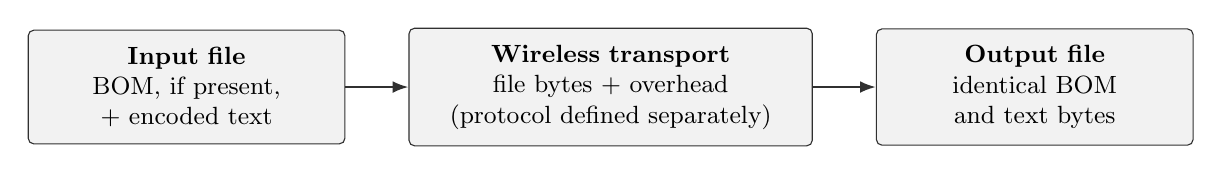
\begin{tikzpicture}[node distance=8mm]
\node[box,text width=36mm] (tx) {\textbf{Input file}\\BOM, if present,\\+ encoded text};
\node[box,text width=47mm,right=of tx] (net) {\textbf{Wireless transport}\\file bytes + overhead\\(protocol defined separately)};
\node[box,text width=36mm,right=of net] (rx) {\textbf{Output file}\\identical BOM\\and text bytes};
\draw[arr] (tx) -- (net);
\draw[arr] (net) -- (rx);
\end{tikzpicture}
\end{center}

\topic{2. Byte order mark}
A plain \code{.txt} file has no mandatory universal header. It may begin with a \textbf{byte order mark (BOM)}, the encoded value U+FEFF used as an encoding signature. In UTF-16 and UTF-32, the BOM also indicates byte order. When interpreted as a BOM, it is not part of the displayed text.

\begin{tabularx}{\linewidth}{@{}P{23mm}P{33mm}Y@{}}
\toprule
\textbf{Encoding} & \textbf{Initial BOM bytes} & \textbf{Meaning for a text decoder}\\
\midrule
UTF-8 & \code{EF BB BF} & Encoding signature only. UTF-8 has no little-/big-endian variants.\\
UTF-16 LE & \code{FF FE} & Read 16-bit units, least-significant byte first.\\
UTF-16 BE & \code{FE FF} & Read 16-bit units, most-significant byte first.\\
UTF-32 LE & \code{FF FE 00 00} & Read 32-bit units, least-significant byte first.\\
UTF-32 BE & \code{00 00 FE FF} & Read 32-bit units, most-significant byte first.\\
\bottomrule
\end{tabularx}

For example, A (U+0041) is stored as \code{41} in UTF-8, \code{41 00} / \code{00 41} in UTF-16 LE/BE, and \code{41 00 00 00} / \code{00 00 00 41} in UTF-32 LE/BE.

\topic{3. Encoding identification}
For an unlabelled text file, the initial BOM normally identifies the encoding. Four-byte signatures are checked before two-byte signatures, followed by strict validation of the encoded text. Transfer and storage preserve the BOM in its original position, regardless of the decoding result.

The absence of a BOM does not identify UTF-8. UTF-16 and UTF-32 files may also omit it. For instance, \code{41 00} represents A followed by NUL in UTF-8, or A in UTF-16 LE. Selecting UTF-8 by default requires an explicit agreement about the input format.

Some signatures overlap. The bytes \code{FF FE 00 00 41 00 00 00} represent either a UTF-32 LE BOM followed by A, or a UTF-16 LE BOM followed by NUL, A and NUL. Checking the longest signature first selects UTF-32 LE, but both interpretations are valid. A declared encoding or an agreed file convention resolves this case.

Character and line processing require a known encoding. A separate copy of the file is decoded with strict error handling, consuming only the initial BOM when applicable. The saved original retains all bytes, including the BOM and line endings. Missing or conflicting encoding information must be resolved before text processing.

\clearpage
\topic{4. File input and output}
The source is opened in binary mode (\code{rb}). The receiver writes the recovered file bytes in their original order, excluding transport headers and padding. The filename and filesystem metadata are stored separately from file content. The transport header format is outside the scope of this report.

The following Python example writes recovered data on a PC. The sequence \code{ordered\_file\_chunks} contains only file bytes. Mode \code{xb} creates a new binary file and fails if the destination already exists.
{\small
\begin{verbatim}
with open(new_path, "xb") as output:
    for chunk in ordered_file_chunks:
        if output.write(chunk) != len(chunk):
            raise OSError("Incomplete file write")
\end{verbatim}
}
The embedded implementation needs equivalent binary filesystem operations and error checks for reading, writing and closing. Buffered data must be flushed and the USB safely unmounted before removal. The saved byte count and contents are checked against the source. Text processing operates on a decoded copy, leaving the received file unchanged.

\topic{5. File reading and chunk boundaries}
File access uses the operating system's filesystem API, or the filesystem library on an embedded platform. Binary reads return bytes without selecting a text encoding. For text processing, the application checks the first four file bytes, or fewer for a shorter file, against the BOM signatures and selects the corresponding decoder. An absent or ambiguous BOM requires a declared encoding or an agreed input format. Decoding does not alter the bytes transferred or saved.

A binary read may split a multibyte character. The text \code{A\'{e}} followed by a CRLF line ending occupies eight bytes in UTF-8 with a BOM. Reading five bytes and then three divides the two-byte representation of \'{e} across the reads.

\begin{center}
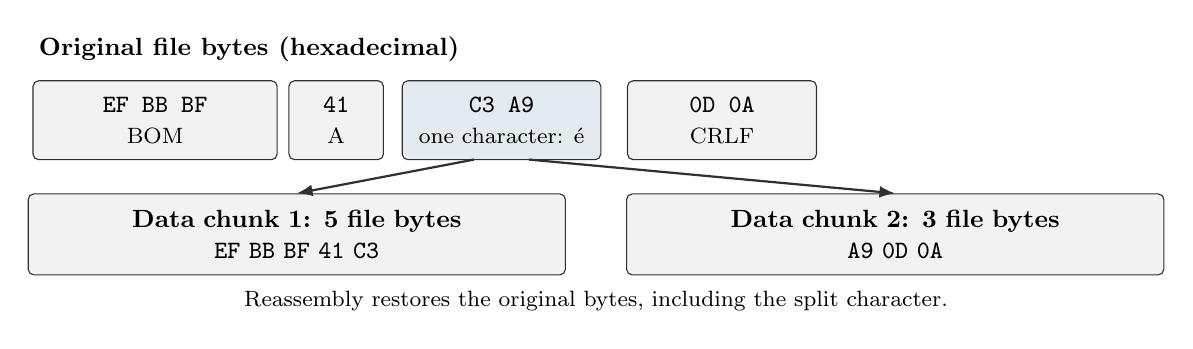
\begin{tikzpicture}[x=1cm,y=1cm]
\node[anchor=west,font=\small\bfseries] at (0,3.0) {Original file bytes (hexadecimal)};
\node[box,minimum width=3.1cm] at (1.6,2.1) {\code{EF BB BF}\\\footnotesize BOM};
\node[box,minimum width=1.2cm] at (3.9,2.1) {\code{41}\\\footnotesize A};
\node[box,fill=accent,minimum width=2.3cm] at (6.0,2.1) {\code{C3 A9}\\\footnotesize one character: \'{e}};
\node[box,minimum width=2.4cm] at (8.8,2.1) {\code{0D 0A}\\\footnotesize CRLF};
\node[box,text width=64mm] (p1) at (3.4,0.65) {\textbf{Data chunk 1: 5 file bytes}\\\code{EF BB BF 41 C3}};
\node[box,text width=64mm] (p2) at (11.0,0.65) {\textbf{Data chunk 2: 3 file bytes}\\\code{A9 0D 0A}};
\draw[arr] (5.65,1.6) -- (p1.north);
\draw[arr] (6.35,1.6) -- (p2.north);
\node[font=\footnotesize,align=center] at (7.2,-0.2) {Reassembly restores the original bytes, including the split character.};
\end{tikzpicture}
\end{center}

Text is decoded after reassembly or with an incremental decoder that retains incomplete sequences between reads. Independent decoding of each chunk can fail when a character or BOM crosses a boundary.

\topic{6. File size}
File size includes the encoded text, line endings and any BOM. Transport overhead is additional. Copying the bytes without conversion preserves the original file size.

For 1,000 ASCII letters with a BOM and no line breaks, the file sizes are:

\begin{center}
\begin{tabular}{@{}lrrr@{}}
\toprule
Encoding & Text bytes & BOM bytes & Total file bytes\\
\midrule
UTF-8 & 1,000 & 3 & 1,003\\
UTF-16 LE / BE & 2,000 & 2 & 2,002\\
UTF-32 LE / BE & 4,000 & 4 & 4,004\\
\bottomrule
\end{tabular}
\end{center}

Omitting the BOM gives sizes of 1,000, 2,000 and 4,000 bytes. Byte order does not affect size. The ratios shown apply to ASCII; other character sets produce different byte counts.

\end{document}
